\documentclass[
	classe=$2^{de}$
]{évaluation}

\usetikzlibrary{calc,patterns}

\title{Évaluation}
\date{5 mai 2023}

\begin{document}

\maketitle

\begin{exercice}
	On dispose des deux volumes suivants :
	\begin{center}
		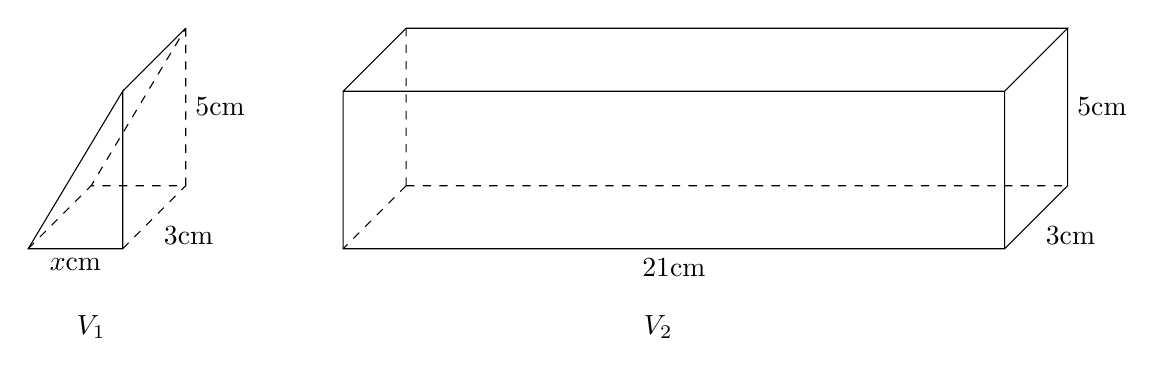
\begin{tikzpicture}[scale=0.4]
			\coordinate (StartA) at (0,0);
			\coordinate (StartB) at (7,0);
			\draw (StartA) -- ++(0,-5) -- node[below] {$x$cm} ++(-3,0)  -- cycle -- ++(2,2);
			\draw[dashed] ($(StartA) + (2,2)$) -- node[right] {$5$cm} ++(0,-5) -- ++(-3,0)  -- cycle
			($(StartA) + (0,-5)$) -- node[below right] {$3$cm} ++(2,2)
			($(StartA) + (-3,-5)$) -- ++(2,2);

			\node at (-1,-7.5) {$V_1$};

			\draw (StartB) -- ++(21,0) -- ++(2,2) -- ++(-21,0) -- (StartB) -- ++(0,-5) -- node[below] {$21$cm} ++(21,0) -- ++(0,5)
			($(StartB) + (21,-5)$) -- node[below right] {$3$cm} ++(2,2) -- node[right] {$5$cm} ++(0,5);
			\draw[dashed] ($(StartB) + (2,-3)$) -- ++(21,0)
			($(StartB) + (2,-3)$) -- ++(-2,-2)
			($(StartB) + (2,-3)$) -- ++(0,5);

			\node at (17,-7.5) {$V_2$};
		\end{tikzpicture}
	\end{center}

	Pour quelle valeur de $x$ le volume de $V_1$ est-il le même que celui de $V_2$ ?
\end{exercice}

\begin{exercice}
	$ABCD$ est un carré de $8$ mètres de côté. On définit sur ses côtés quatres points $E$, $F$, $G$ et $H$ tels que $DE = CF = BG = AH = x$ (en mètres), comme sur la figure ci-dessous.

	On veut trouver la ou les valeurs de $x$ telle(s) que la surface hachurée ai une aire de $32\text{m}^2$.
	\begin{center}
		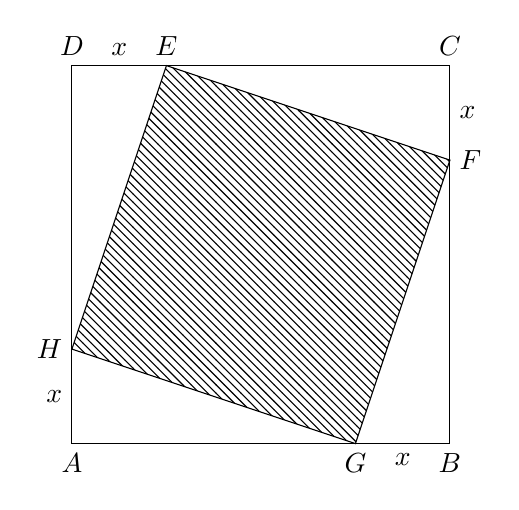
\begin{tikzpicture}[scale=0.6]
			\pgfmathsetmacro\x{2}
			\coordinate (A) at (0,0);
			\coordinate (B) at (8,0);
			\coordinate (C) at (8,8);
			\coordinate (D) at (0,8);
			\coordinate (H) at ($(A) + (0,\x)$);
			\coordinate (G) at ($(B) + (-\x,0)$);
			\coordinate (F) at ($(C) + (0,-\x)$);
			\coordinate (E) at ($(D) + (\x,0)$);
			\foreach \p in {A,B,G} {
					\node[below] at (\p) {$\p$};
				}
			\foreach \p in {C,D,E} {
					\node[above] at (\p) {$\p$};
				}
			\node[right] at (F) {$F$};
			\node[left] at (H) {$H$};
			\node[above] at ($(D)!0.5!(E)$) {$x$};
			\node[right] at ($(C)!0.5!(F)$) {$x$};
			\node[below] at ($(G)!0.5!(B)$) {$x$};
			\node[left] at ($(A)!0.5!(H)$) {$x$};
			\draw (A) -- (B) -- (C) -- (D) -- cycle;
			\draw[pattern=north west lines] (E) -- (F) -- (G) -- (H) -- cycle;
		\end{tikzpicture}
	\end{center}

	\begin{enumerate}
		\item Déterminer l'aire $a(x)$ du triangle $AGH$ en fonction de $x$ (en mètres carrés), et vérifier qu'elle peut s'écrire $a(x) = 8 - \dfrac{1}{2}(x - 4)^2$.
		\item Résoudre le problème posé dans l'énoncé.
	\end{enumerate}
\end{exercice}

\begin{exercice}
	\begin{enumerate}
		\item À l'aide d'une calculatrice, donner l'arrondi au millième près des deux nombres suivants :
		      \begin{align*}
			      A & = \dfrac{\sqrt{7} - \sqrt{5}}{\sqrt{2}} & B & = \dfrac{\sqrt{2}}{\sqrt{5} + \sqrt{7}}
		      \end{align*}
		\item Quelle conjecture peut-on faire concernant ces deux nombres ?
		\item Mettre les fractions sur le même dénominateur pour prouver cette conjecture.
	\end{enumerate}
\end{exercice}

\begin{exercice}
	On s’intéresse au problème suivant : « Quels sont les nombres entiers naturels qui peuvent s’écrire comme différence de deux carrés d’entiers ? »
	\begin{enumerate}
		\item \begin{enumerate}
			\item Développer et réduire $(n + 1)^2 - n^2$ puis $(n + 1)^2 - (n – 1)^2$.
			\item Montrer que tout nombre impair peut s’écrire comme la différence de deux carrés.
			\item Montrer que tout multiple de $4$ peut s’écrire comme la différence de deux carrés.
		\end{enumerate}
		\item Réciproquement, soient $x$ et $y$ deux entiers naturels et soit $N = x^2 - y^2$.
		
		Montrer que $N$ est soit un nombre impair, soit un multiple de $4$ (on pourra étudier les différents cas selon la parité de $x$ et de $y$).
	\end{enumerate}
\end{exercice}

\end{document}